\section{Management}

\subsection{Document Store}

\paragraph{NoSQL}
Nestedness and heterogeneity. Joins are hard. Document-oriented DBs are one of the main categories of NoSQL

\paragraph{Document Store}
Storing many small documents (e.g. JSON/XML documents = "record") a.k.a a collection of trees (tree per document) a.k.a semi-structured data. Validate after data was populated. MongoDB is one implementation of a document store.

\paragraph{Encodings (Char to 0/1)}
\begin{itemize}
    \item ASCII
    \item ISO Latin 1
    \item UTF-8
    \item UTF-16
\end{itemize} %TODO, bson


\subsection{MongoDB}

See reading assignment "MongoDB: The Definitive Guide".

\paragraph{Introduction}
MongoDB is a document-oriented DB program - classified as NoSQL. It uses JSON-like documents with optional schemas. Main features include:
\begin{itemize}
    \item Ad-hoc queries such as point queries, range queries and regex searches. Queries can return specific fields of documents.
    \item Fields in a document can be indexed (primary on \_id and secondary on other fields).
    \item Data is replicated to provide high availability. Writes and reads are done on primary replica, secondaries maintain a copy (eventual consistency). If primary fails, a new primary is selected.
    \item Horizontal scaling by using sharding. Shard key chosen by user determines how data in collection will be distributed. Data is split into ranges based on key and distributed across multiple shards (=master with one or more replicas). Even distribution with hash partitioning possible. %TODO more on that
    \item MongoDB provides the capability to validate documents during updates and insertions.
    \item There are no joins in MongoDB!
\end{itemize}

%TODO coding. cheat sheet






\paragraph{MongoDB Stack}
See Figure \ref{fig:mdb_stack}.

\begin{figure}[h]
	\centering
	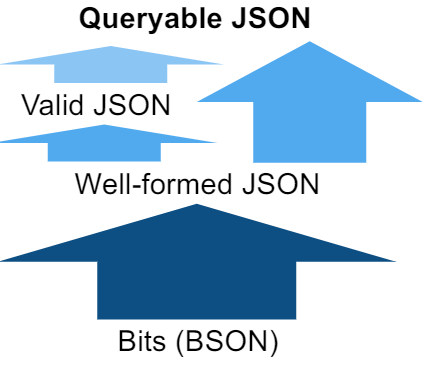
\includegraphics[scale=0.65]{images/5-mdb_stack.PNG}
	\caption{MongoDB Stack.}
	\label{fig:mdb_stack}
\end{figure}

\paragraph{Querying: CRUD}
Create, read, update, delete. Writing atomicity is at document-level. No need for schema until projection. %TODO code? mongodb queries? cheatsheet

\paragraph{Architecture}
%TODO sharding, replication, indices (hash, btree)




%TODO MongoDB reading


mongodb can compare anything with anything

architecture (no hdfs below mongodb!)
- primary nodes, write 3 replicas ACK and then asynch
- 1 doc = 1 tree
- 1 shard = multiple docs


indices
- there have been none until now, we always scan everything (need to be built by the programmer)
- doc stores have indices for programmer
- hash, good for point
- b+ trees, how to create it, good for point and range


mongodb data fits on single machine (usually)




\subsection{Query Languages}

%TODO nestedness and SQL
%TODO JSONiq sandbox



querying trees

jsoniq (data model, operations, data flow, flwor, types)
json navigation (jsoniq, rumble)

query processing, iterative/streamed vs. materialization





\subsubsection{Rumble}

See reading assignment "Rumble: Data Independence for Large Messy Data Sets".

\paragraph{Introduction}
Rumble is a query execution engine for large, heterogeneous and nested collections of JSON objects built on top of Apache Spark (usually running over HDFS). It uses JSONiq as the interface language, which is a standardized language for querying JSON documents.

Rumble shows that data independence for JSON processing is achievable with reasonable performance on top of large clusters.

Other formats are possible (txt, parquet, csv, etc.) and other file systems are possible (local, S3, Azure, etc.).

\paragraph{Issues Rumble Solves}
Values which cannot fit a regular structure are dropped (in table-based tools), nested objects are kept as complete strings or mapped to non-existing values. Simply converting JSON documents to DataFrames is therefore uncool.

\paragraph{JSONiq}
\begin{itemize}
    \item Fit recursive JSON structure on Spark's DataFrames: JSONiq expression is translated into a tree of iterators.
    \item Declarative language.
    \item Manipulating ordered and potentially heterogeneous sequences of items (atomic values, structured items such as objects and arrays, function items).
    \item Sequence: always flat and unnested, separated by comma, can be empty. A sequence of one item is the same as the item itself.
    \item Process each item of a sequence individually with FLWOR expressions (for, let, where, order by, group by, return) - similar to Haskell programming. %TODO more code
\end{itemize}

\paragraph{Query Result}
Results can be displayed, stored to file or written to a distributed file by Spark.

\paragraph{Basic Operations}
%TODO see summary, rel algebra

%TODO cardinality stuff, casting


\paragraph{Precedence}
See Figure \ref{fig:jsoniq_prec}. Use parentheses to override precedence ordering.

\begin{figure}[h]
	\centering
	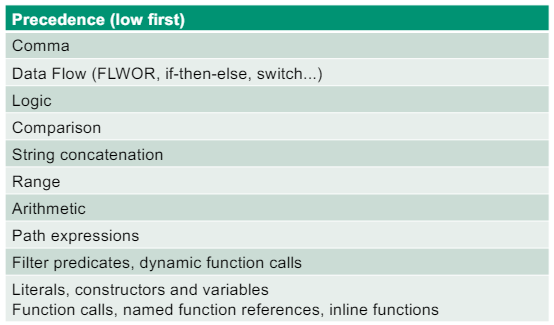
\includegraphics[scale=0.65]{images/5-precedence.PNG}
	\caption{Higher precedence first.}
	\label{fig:jsoniq_prec}
\end{figure}